%!TEX root = ../thesis.tex
%*******************************************************************************
%****************************** Introduction Chapter ***************************
%*******************************************************************************
\chapter{Background}


% outline pandora methods from rachel's thesis
\section{Pandora}
\label{sec:pandora-intro}
%  discuss how pandora decides on presence absence of loci
\cite{rachelthesis}

\subsection{Multi-sample variation inference}
\label{sec:pandora-compare}

% Choice of reference path may disguise small variants with shared flanking
% sequence: for toy local graph in (a) and two samples shown in orange and blue, figures
% (b) and (c) show VCF details describing the SNP difference between these two samples
% with respect to 2 different choices of reference path, shown in black. In (c) the difference is
% explicitly written as a SNP, whilst in (b) it is nested within longer alleles.

\begin{figure}
\begin{center}
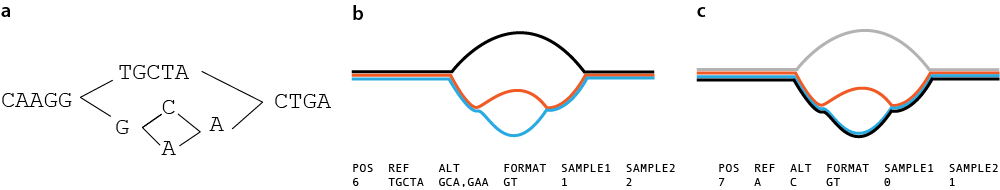
\includegraphics[width=0.95\columnwidth]{Chapter0/Figs/variant_representation.png}
\caption{{An illustration of how the...
{\label{fig:var-representation}}
}}
\end{center}
\end{figure}

\begin{figure}
\centering
\missingfigure{reference bias figure 1b in pandora paper}
\caption{A missing figure}
\label{fig:reference-bias}
\end{figure}

% outline make prg method. make sure to talk about max nesting and min match len

% minimizer kmers

\section{Using genome graph for drug resistance prediction}
\label{sec:genome-graphs-dst}

\drprg{} is not the first tool to use the concept of genome graphs for AMR prediction. mykrobe, the other tool used in this chapter, uses population genome graphs for genotyping of samples. The underlying method mykrobe uses is Cortex \cite{iqbal2012} - a program that uses coloured de Bruijn graphs (dBGs) for genotyping samples via \denovo{} assembly. Cortex is somewhat of a precursor to \pandora{} - the genome graph method underpinning \drprg{}. However, \pandora{} offers a number of advantages over Cortex (see \autoref{sec:genome-graphs-dst} for a full description of these). The first being the representation of the genome graph itself. As mentioned, Cortex uses \kmer{}s in coloured dBGs, while \pandora{} uses minimizing \kmer{}s in a \emph{directed} graph. In the context of \ont{} data, this distinction is important. As we saw in \autoref{chap:denovo}, build dBGs from \ont{} creates very complex graphs. In addition, as the \ont{} error rate is higher than Illumina, a smaller \kmer{} size is required, another factor that increases the complexity of the dBG. Another important difference in the graph representations of Cortex (mykrobe) and \pandora{} (\drprg{}) is the way in which \kmer{} "hits" are encorporated. In a dBG, anywhere that a \kmer{} matches, the depth is incremented by one. However, in \pandora{} such hits are dependent on the context of the read. If a \kmer{} matches two locations in the graph, but one location has many hits close by from the same read while the other does not, the spurious hit is discarded. This filtering of \kmer{} hits allows us to use a lower \kmer{} size ($k=15$) in \pandora{}, and thus \drprg{}, than is used by Cortex/mykrobe ($k=21$). Another flow-on effect of using a smaller \kmer{} size is we do not require as much read depth in \drprg{} as there is a much higher chance of matches to smaller \kmer{}s, especially when the error rate is high. For example, assuming a \ont{} error rate of 0.08, we would expect the probability of a $15-mer$ and $21-mer$ having no errors to be 0.30 and 0.19 respectively. A more in-depth discussion of the differences between these graph methods can be found in (LINK\todo{link to intro section discussing cortex/pandora differences}).

%  nanopore sequencing
% how does it work
% history of basecallers